\chapter{Prototype Design}
This chapter focuses on the design of the prototype of the NeoPixel Sunrise Clock (NPSC). It starts by providing an overview of the NPSC system design, followed by a high-level description of the sub-systems design and a detailed design of the hardware modules. The system design provides an overview of the NPSC's module. The high-level design focuses on the thinking process behind the design of the applications at level 3 of the system hierarchy. The detailed design focuses on the hardware modules at level 1 of the system hierarchy, providing more detailed on the design of the hardware.

%%%%%%%%%%%%%%%%%%%%%%%%%%%%%%%%%%%%%%%%%%%%%%%%%%%%%%%%%%%%%%%%%%%%%%%%%%%%%%%%%%%%
% SECTION: System design
%%%%%%%%%%%%%%%%%%%%%%%%%%%%%%%%%%%%%%%%%%%%%%%%%%%%%%%%%%%%%%%%%%%%%%%%%%%%%%%%%%%%
\section{System design}
The system requirements of the NPSC are the following:
\begin{itemize}
\item The NPSC should be able to emit light and simulate sunrise. 
\item The NPSC should be able to display time and set alarms.
\item The NPSC should be controllable using a touchscreen device.
\end{itemize}
These system requirements are achieved by the functions of the applications at level 3 of system modular hierarchy illustrated in \cref{fig:system_hierarchy}. Each application focuses on one requirement but might involve other requirements, the relations between some hardware modules and their application module are illustrated by \cref{fig:system_overview} and explained below.
\begin{figure}[ht]
\centering
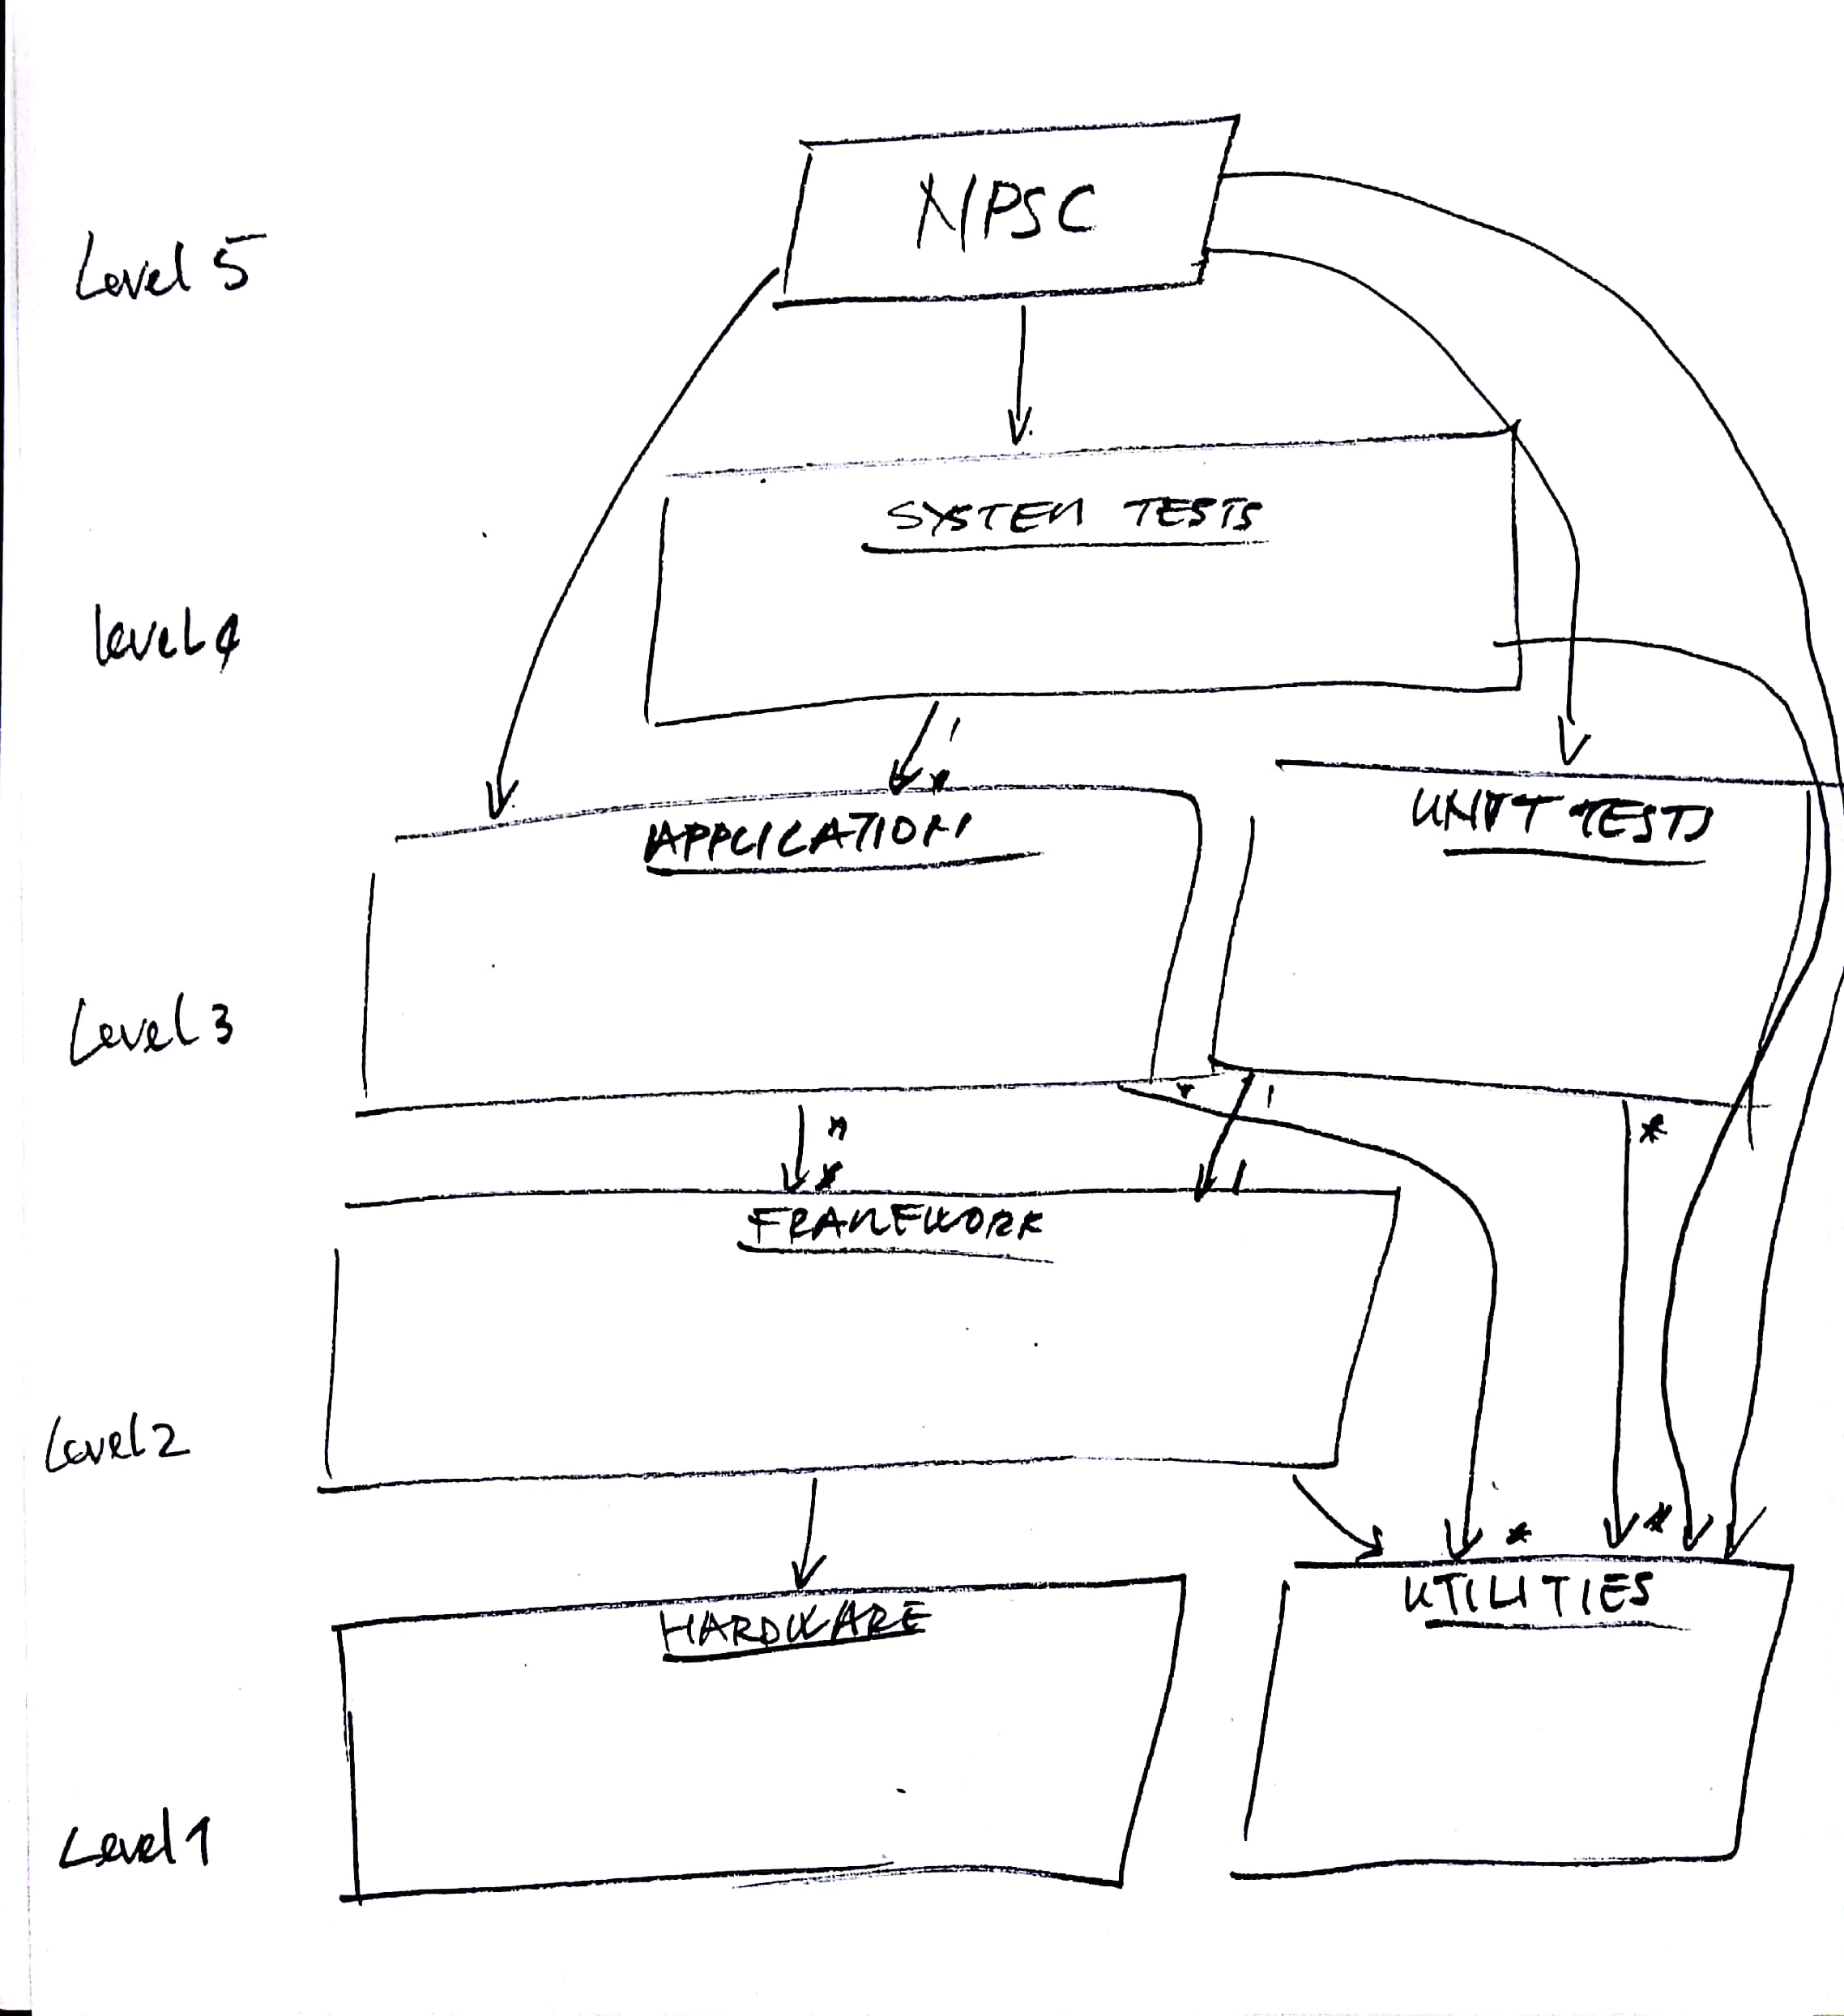
\includegraphics[scale=0.11]{system_overview.jpg}
\caption{Detailed structural block diagram of the NPSC showing the connections between the hardware modules and the main software modules.}
\label{fig:system_overview}
\end{figure}
\begin{itemize}
\item \textbf{Visual application}: This application controls the \textit{Ring}, \textit{Time}, \textit{Weekday}, and \textit{Date} PCBs. It manages visual outputs hardware, from setting the brightness to ensuring that a specific pattern is displayed to ensuring that the desired lux quantity is emitted by the NPSC.
\item \textbf{Alarm application}: This application manages the synchronisation of the internal and external clocks. It is also responsible for managing the alarm stored in the EEPROM and updating the alarm.
\item \textbf{Instruction Queue application}: This application is responsible for the creation of instructions from the user input devices (Nextion touchscreen and Smartphone application) and manages the instruction queue.
\item \textbf{Instruction Fetch Decode and Execute (IFDE) application}: This application relies on the result of the instruction queue application. The IFDE fetches instructions from the instruction queue, decode the instructions and execute commands based on the instruction's opcode. It is the bridge between the user inputs and the hardware modules of the NPSC.
\end{itemize}

%%%%%%%%%%%%%%%%%%%%%%%%%%%%%%%%%%%%%%%%%%%%%%%%%%%%%%%%%%%%%%%%%%%%%%%%%%%%%%%%%%%%
% SECTION: High-level Design
%%%%%%%%%%%%%%%%%%%%%%%%%%%%%%%%%%%%%%%%%%%%%%%%%%%%%%%%%%%%%%%%%%%%%%%%%%%%%%%%%%%%
\section{High-level design}
This section provides more detailed explanation of the system design requirements broken down into sub-system design requirements. The sub-systems requirements are listed below:
\begin{itemize}
\item Control light pattern
\item Control light parameters
\item Update and obtain time and date from clock
\item Set, edit alarms
\item Store user preferences
\item Control the NPSC using an onboard touchscreen
\item Control the NPSC using a smartphone application
\end{itemize}
The following sections explain the design of the main modules of the NPSC created to meet the system and sub-system requirements.

\subsection{Inputs/Outputs instruction design}
This section focuses on the design of the user inputs capture and interpretations. \Cref{fig:io_instruction} shows the communication between the microcontroller and the inputs, and the different step through which information sent by these inputs are analysed. 
\begin{figure}[ht]
\centering
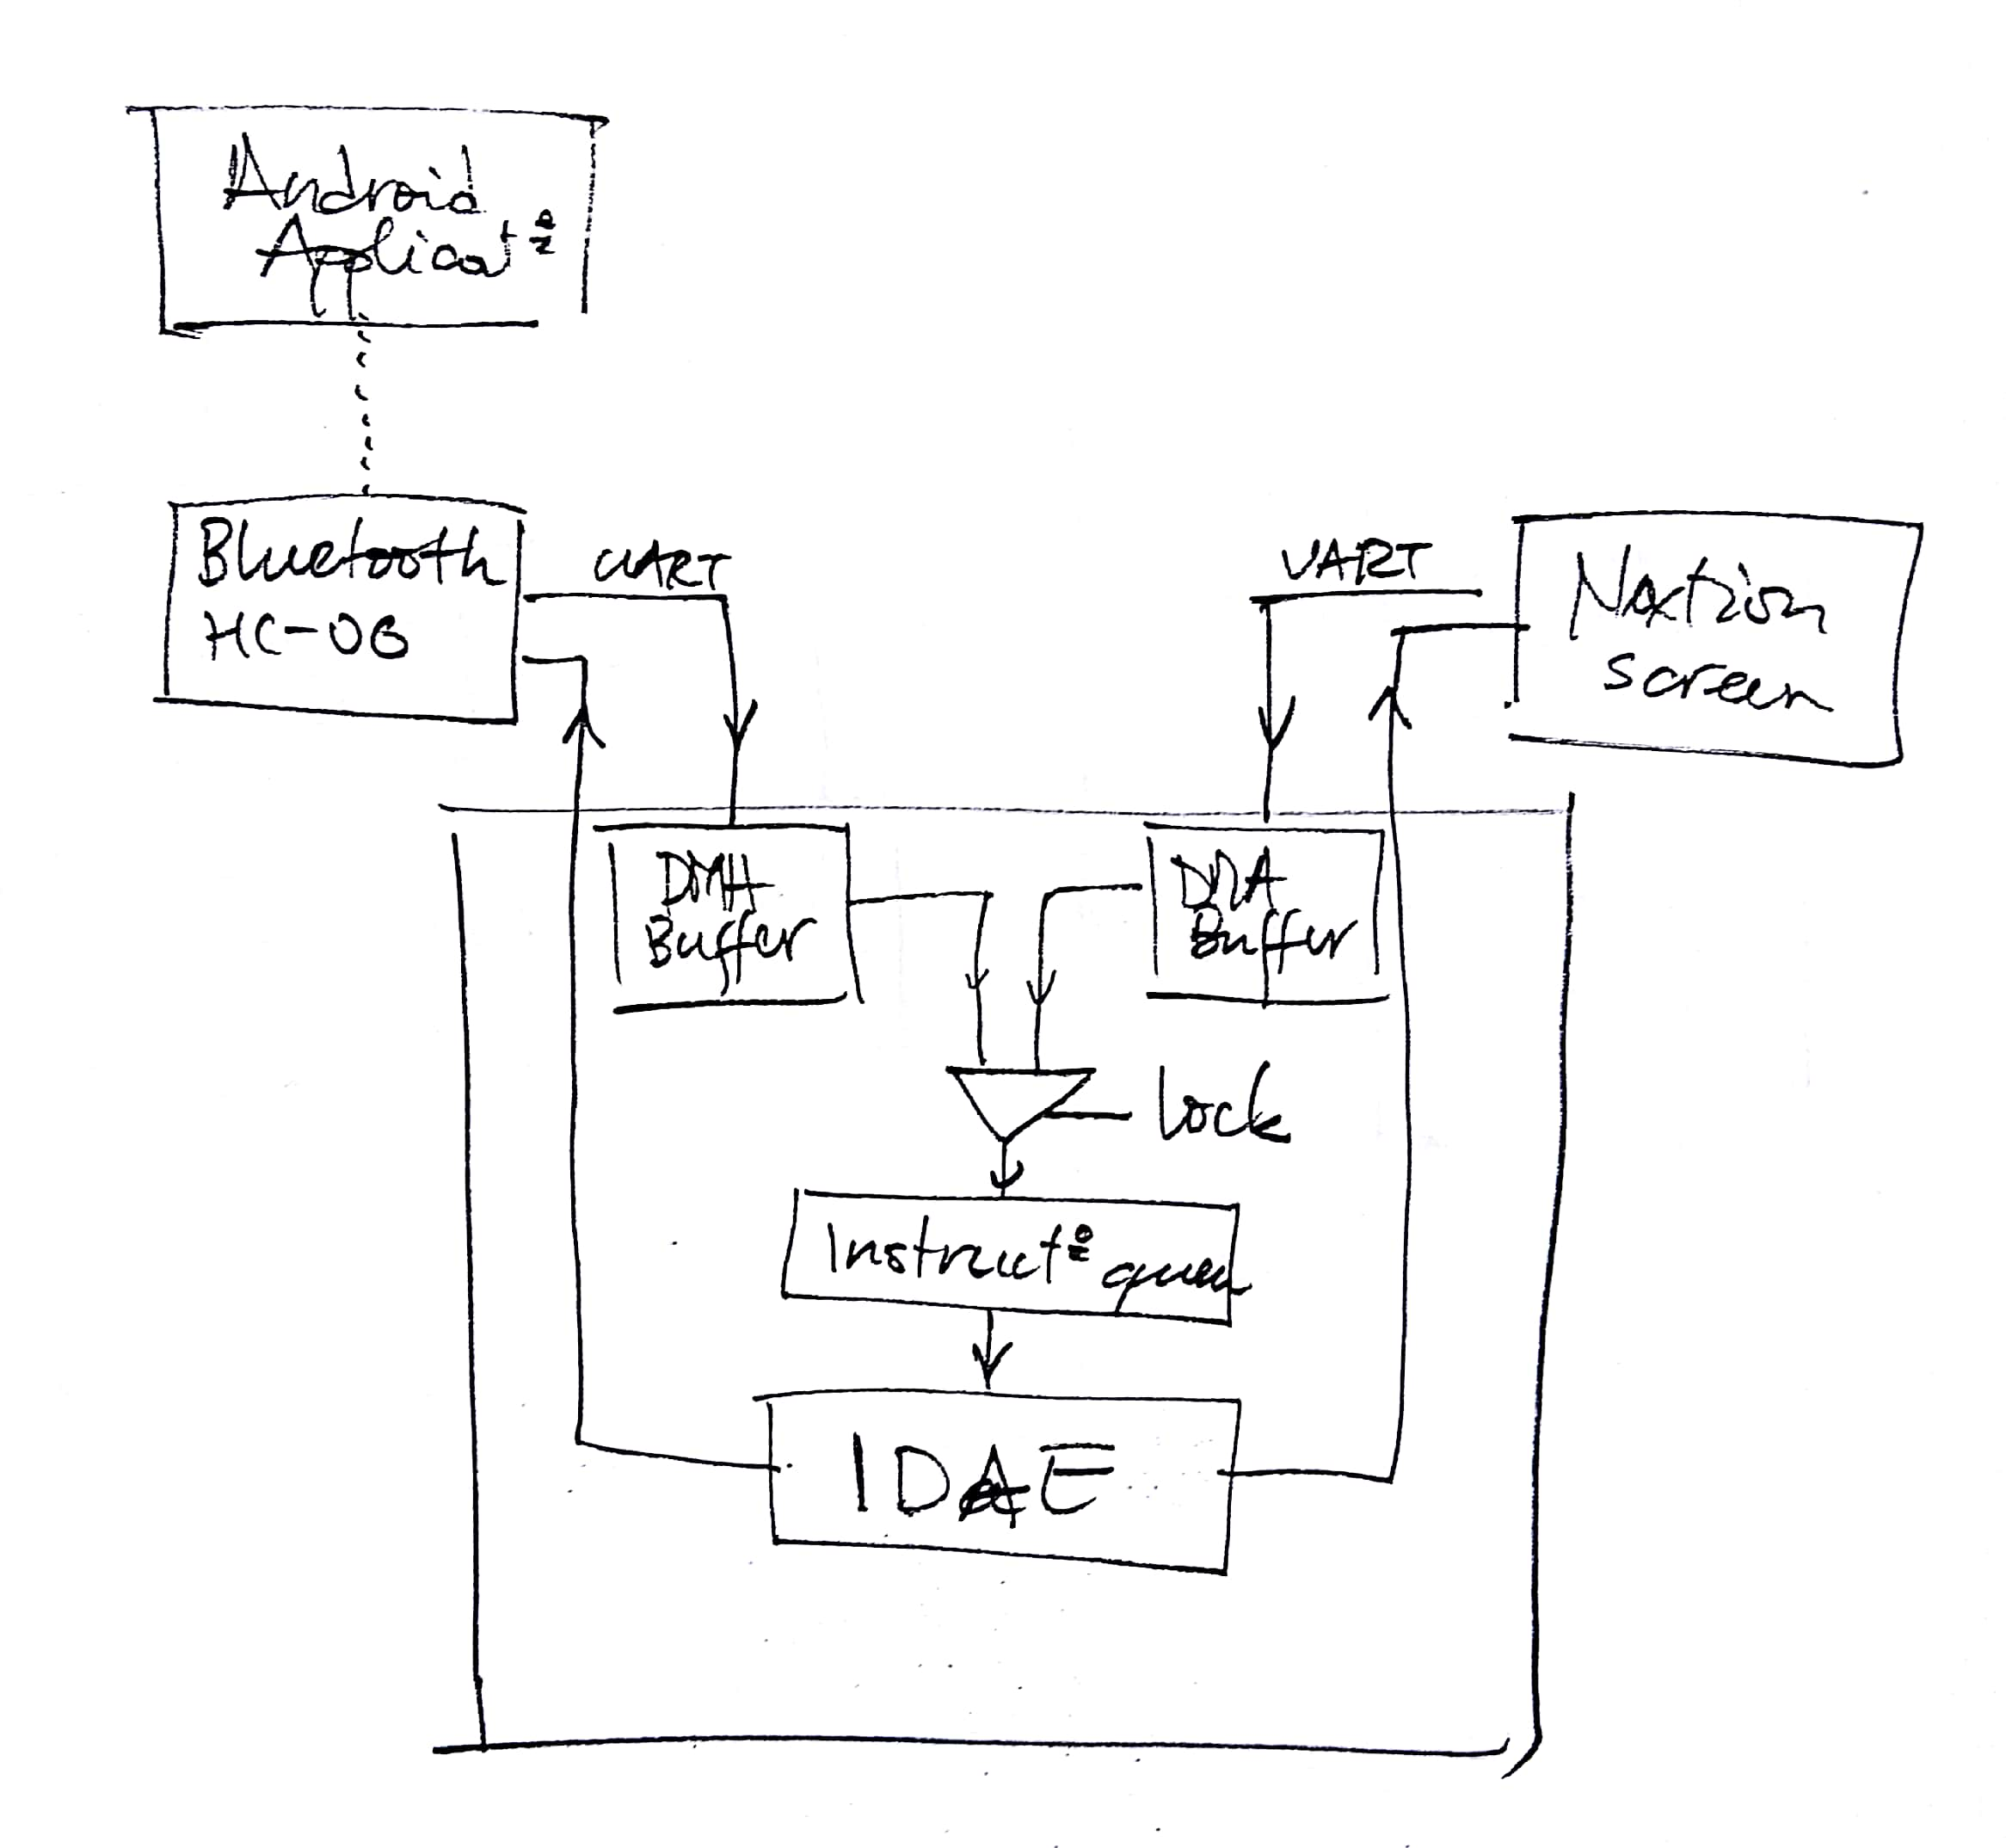
\includegraphics[scale=0.15]{io_instruction.jpg}
\caption{}
\label{fig:io_instruction}
\end{figure}

\subsubsection{From the inputs to the microcontroller}
There are two user inputs, a smartphone application running on an android device and a nextion screen. The android application communicates with the microcontroller via Bluetooth. Both the Bluetooth device and the Nextion touchscreen use the Universal Asynchronous Receiver-Transmitter (UART) protocol to communicate with the micro. Because the instructions are more than one byte, the microcontroller must be able to receive a stream of bytes with no information loss.\\
To achieve this, each UART uses the Direct Memory Access (DMA) to store each stream received to the corresponding DMA Buffer. After the reception of a stream of data, each DMA Buffer converts its data into instructions which are added to the instruction queue.\\
The DMA function is called on interrupt when the microcontroller receives data on the DMA channel. For this reasons it might occur that one DMA pauses the addition of instruction to the instruction queue by another DMA, and start adding new instructions to the queue. This is a potential concurrency problem that can corrupt the instructions added to the queue. To solve this problem, the addition of instruction to the queue is considered as a critical section of the design. A lock is thus added to the instruction queue such that only a process owning the lock can add new instructions to the queue.\\
The instruction queue is a First In First Out (FIFO) queue, meaning that an element removed from the queue was the oldest element in the queue. This allows the instruction to be executed in order of arrival.

\subsubsection{Instruction Fetch Decode Execute (IFDE)}
The IFDE act as the Central Processing Unit (CPU) of the NPSC. Its role is to fetch instructions from the instruction queue, decode the instructions and execute them by calling the corresponding methods. It is the brain of the NPSC operation and acts as a bridge between the user inputs and the different hardware module. As the IFDE uses specific instruction set, there is a restriction on the actions performed by the users reducing any security breaches. By using an instruction set and the IFDE, the functionalities of the NPSC can easily be expanded and modify during the software development.
 
\subsubsection{Buffer size and Instruction sets}
The instruction size was mostly defined by the rules of the Nextion touchscreen. This touchscreen is able to send information to a microcontroller using UART. However, it does not send a single byte of data unless a character is sent. As it is not convenient to convert all the integer parameters into characters, the second build-in method used by the nextion to send information was considered. This method sends an integer value as four bytes of data. Because certain methods of the framework require structs \footnote{A struct also known as a record is a collection of data type used to represent entities having multiple attributes} as parameters, the instruction size was set to be double the size of the number of bytes sent by the nextion touchscreen per each method call. \\
The DMA Buffer size is dependent on the design of the Nextion touchscreen application and the Android application, as a stream of instruction might be sent. The number of instructions in the queue is also dependent on the DMA Buffer size because there are two inputs and therefore two DMAs, a rule of thumb for the instruction queue size is to be at least the number of inputs multiply by the DMA Buffer size.\\

The instructions of the NPSC are listed in \cref{table:instruction_set}. The instructions are divided into categories, each category represent the actions performed at a framework level or application level (see \cref{fig:system_hierarchy}). There are two types of instructions, the set instructions and the get instructions. The set instructions write informations to the NPSC while the get information are just signal indicating that the user input device is requesting information. The instrcutions are 8 bytes long and the first byte represent the opcode of the instrucion while other byte are for the data sent. Instructions of the same category have the same most significant four bytes, for example all intructions from the Alarm category have $0x1*$ as their opcode with $*$ being any one digit hexadecimal number. The pcode 0x00 is reserved for identifying data that must not be converted into instructions.
\begin{landscape}
\begin{table}[t!]
\centering
\begin{tabular}{cccccccccc}
\hline
\hline
\multicolumn{10}{c}{Instructions} \\
\toprule
\multirow{2}{*}{Category} & \multirow{2}{*}{Name} & \multicolumn{8}{c}{Instruction bytes} \\
& & \textbf{M0/opcode} & \textbf{M1} & \textbf{M2} & \textbf{M3} & \textbf{M4} & \textbf{M5} & \textbf{M6} & \textbf{M7} \\
\hline
\toprule
\multirow{2}{*}{External RTC} & set clock & \textbf{0x01} & year & month & date & weekday & hour & minute & second \\
& get clock & \textbf{0x02} & - & - & - & - & - & - & - \\
\midrule
\multirow{6}{*}{Alarm} & set alarm time parameters & \textbf{0x10} & id & hour & minute & date/day selection & day/date & repeat & - \\
& set alarm extra parameters & \textbf{0x11} & id & ringtone & pattern & enable & fetch & - & - \\
& set alarm label & \textbf{0x12} & id & label number & - & * & * & * & * \\
& set alarm enable & \textbf{0x13} & id & enable & - & - & - & - & - \\
& get alarm minimum parameters & \textbf{0x14} & id & id & - & - & - & - & - \\
& get alarm parameters & \textbf{0x15} & id & - & - & - & - & - & - \\
\bottomrule
\hline
\end{tabular}
\caption{Instruction set used for the control of the NPSC by the users. Each instruction has a category, a name and an opcode. \textbf{-} in the table indicates data that will not be used by the IFDE. \textbf{*} indicates character data.}
\label{table:instruction_set}
\end{table}
\end{landscape}

\subsection{External storage}
The storage's purpose is to store useful information such as the alarm parameters and the user's preferences. Certain application require storage capability, therefore there is a restricted access to the EEPROM memory. The memory allocation is detailed in \cref{fig:eeprom}.
\begin{figure}[ht]
\centering
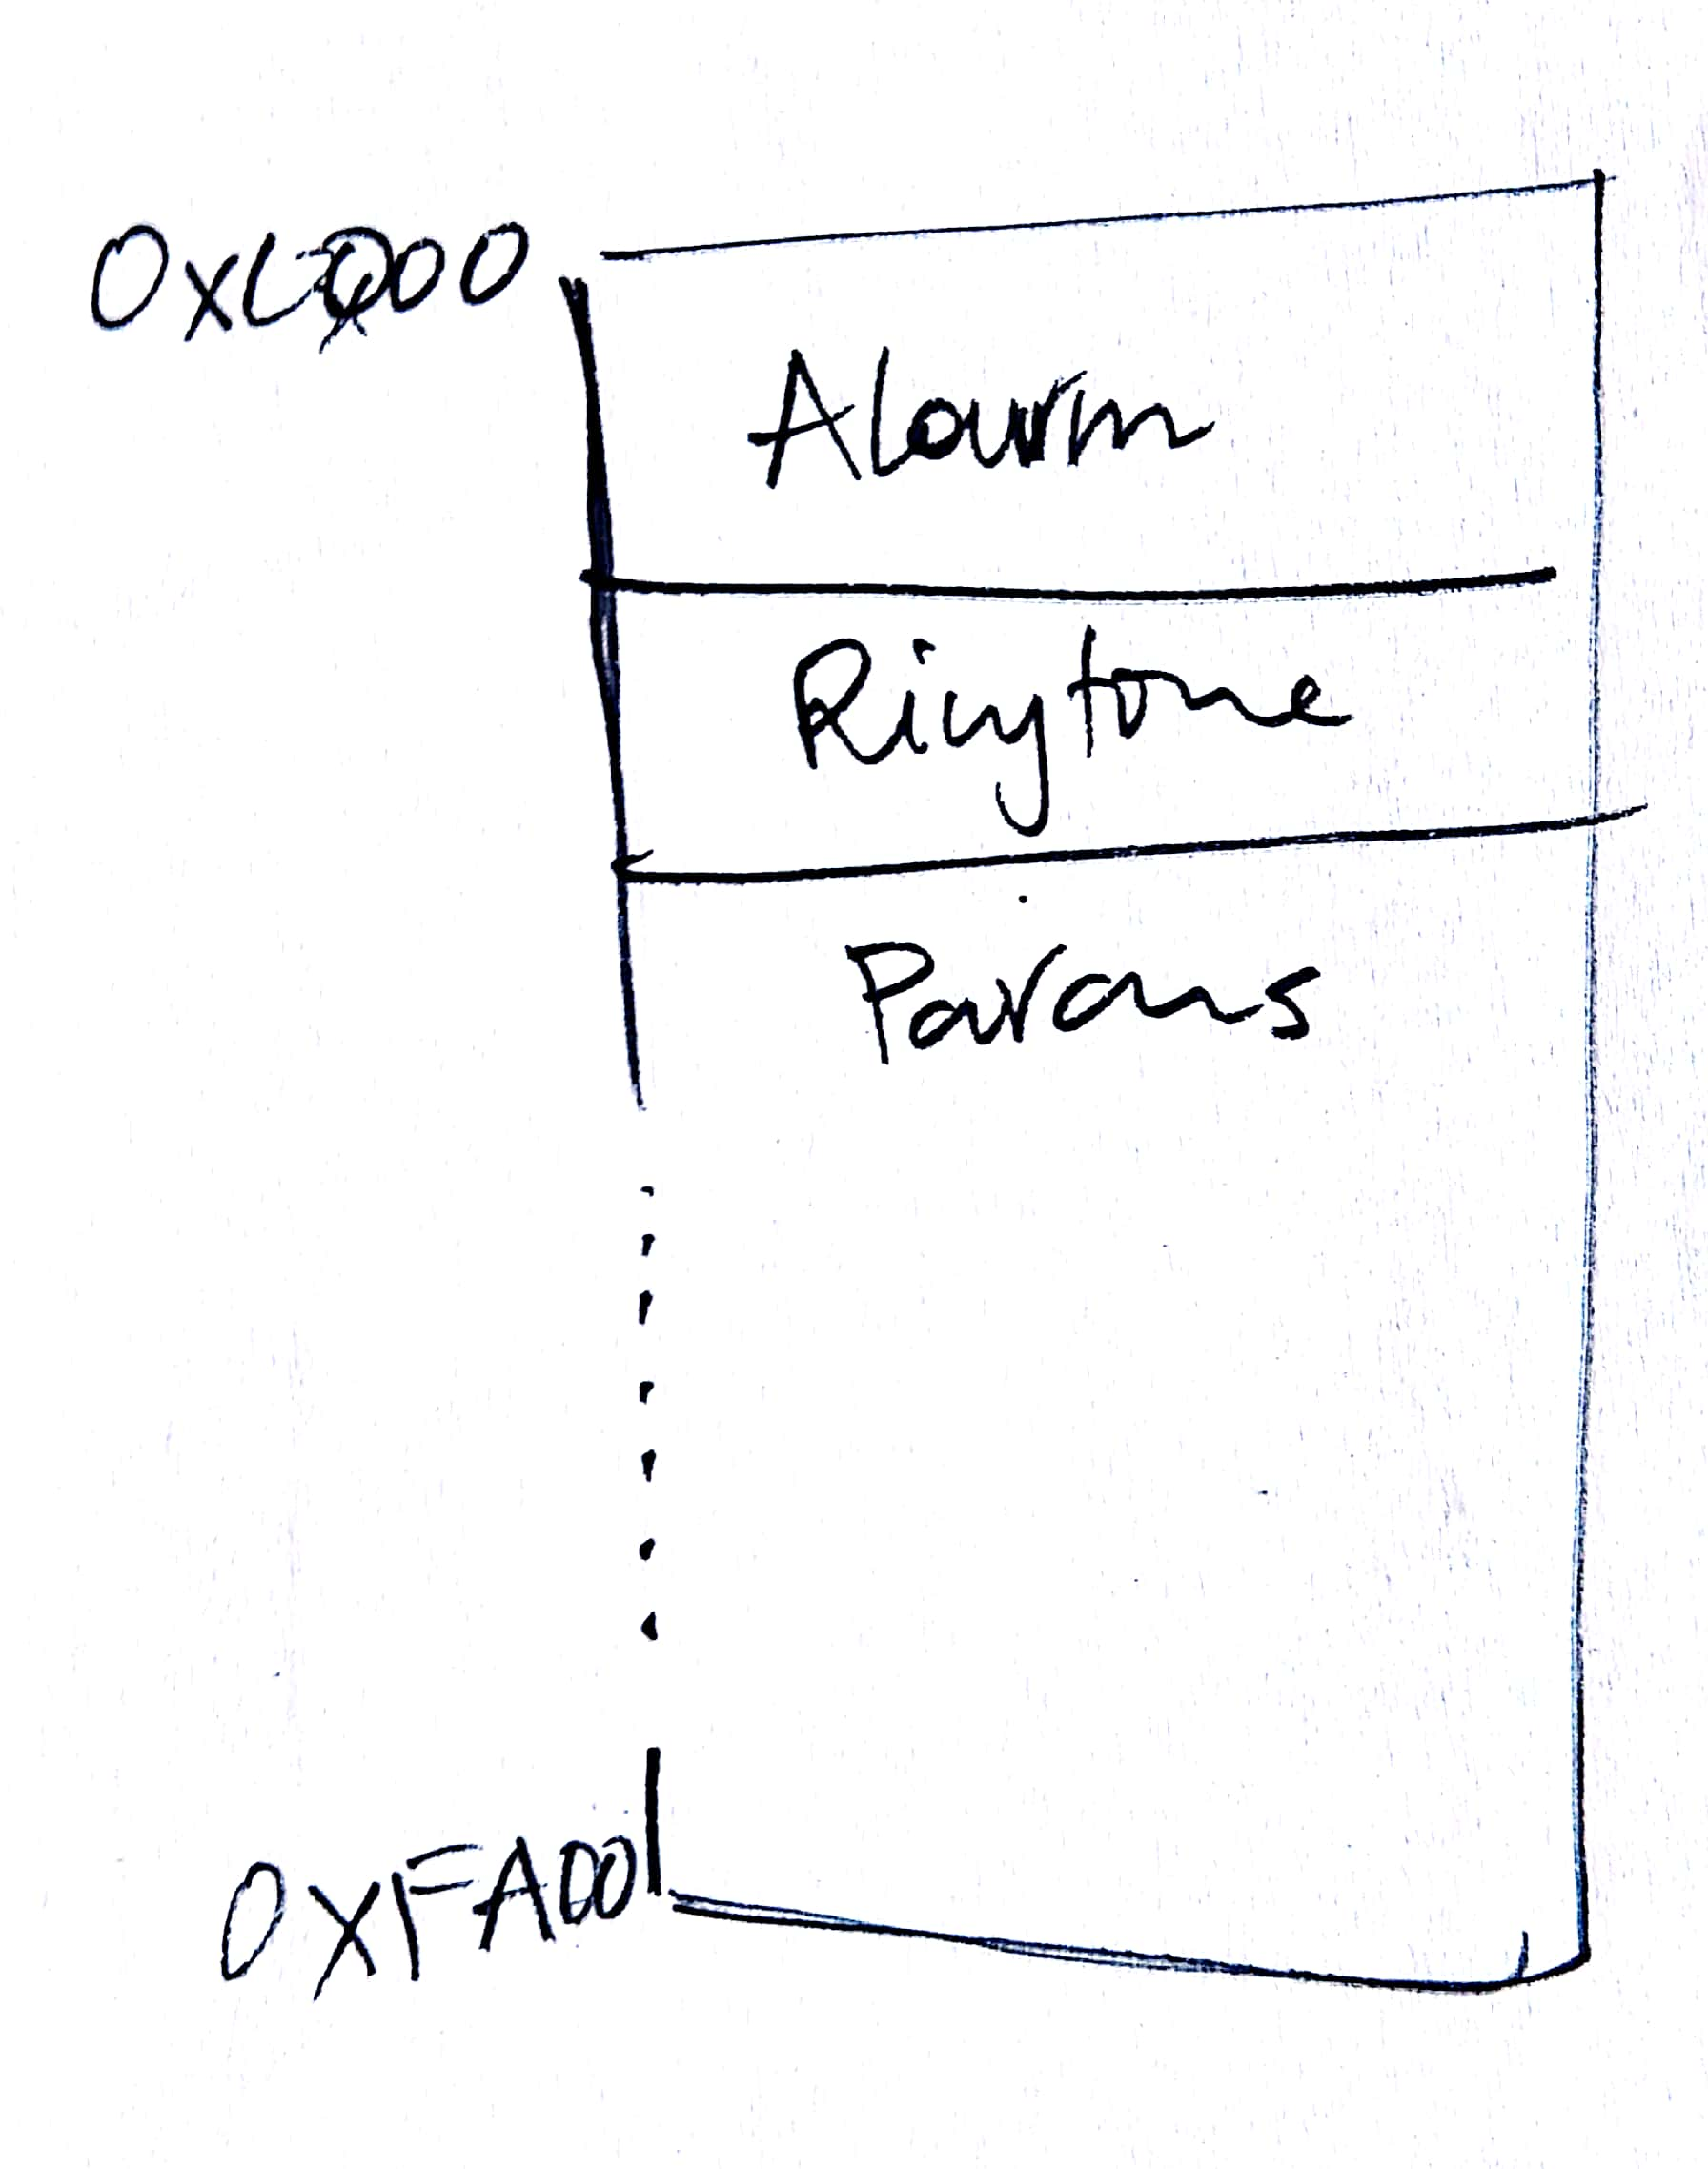
\includegraphics[scale=0.08]{eeprom.jpg}
\caption{}
\label{fig:eeprom}
\end{figure}

\subsection{Alarm and Clock}
The structural diagram of this module is shown in \cref{fig:alarm_clock}. The microcontroller used by the NPSC has a built-in RTC with two alarms (alarm A and alarm B), this module makes use of an Alarm manager (application software) which control the EEPROM, the external and internal RTCs and the two alarms.
\begin{figure}[ht]
\centering
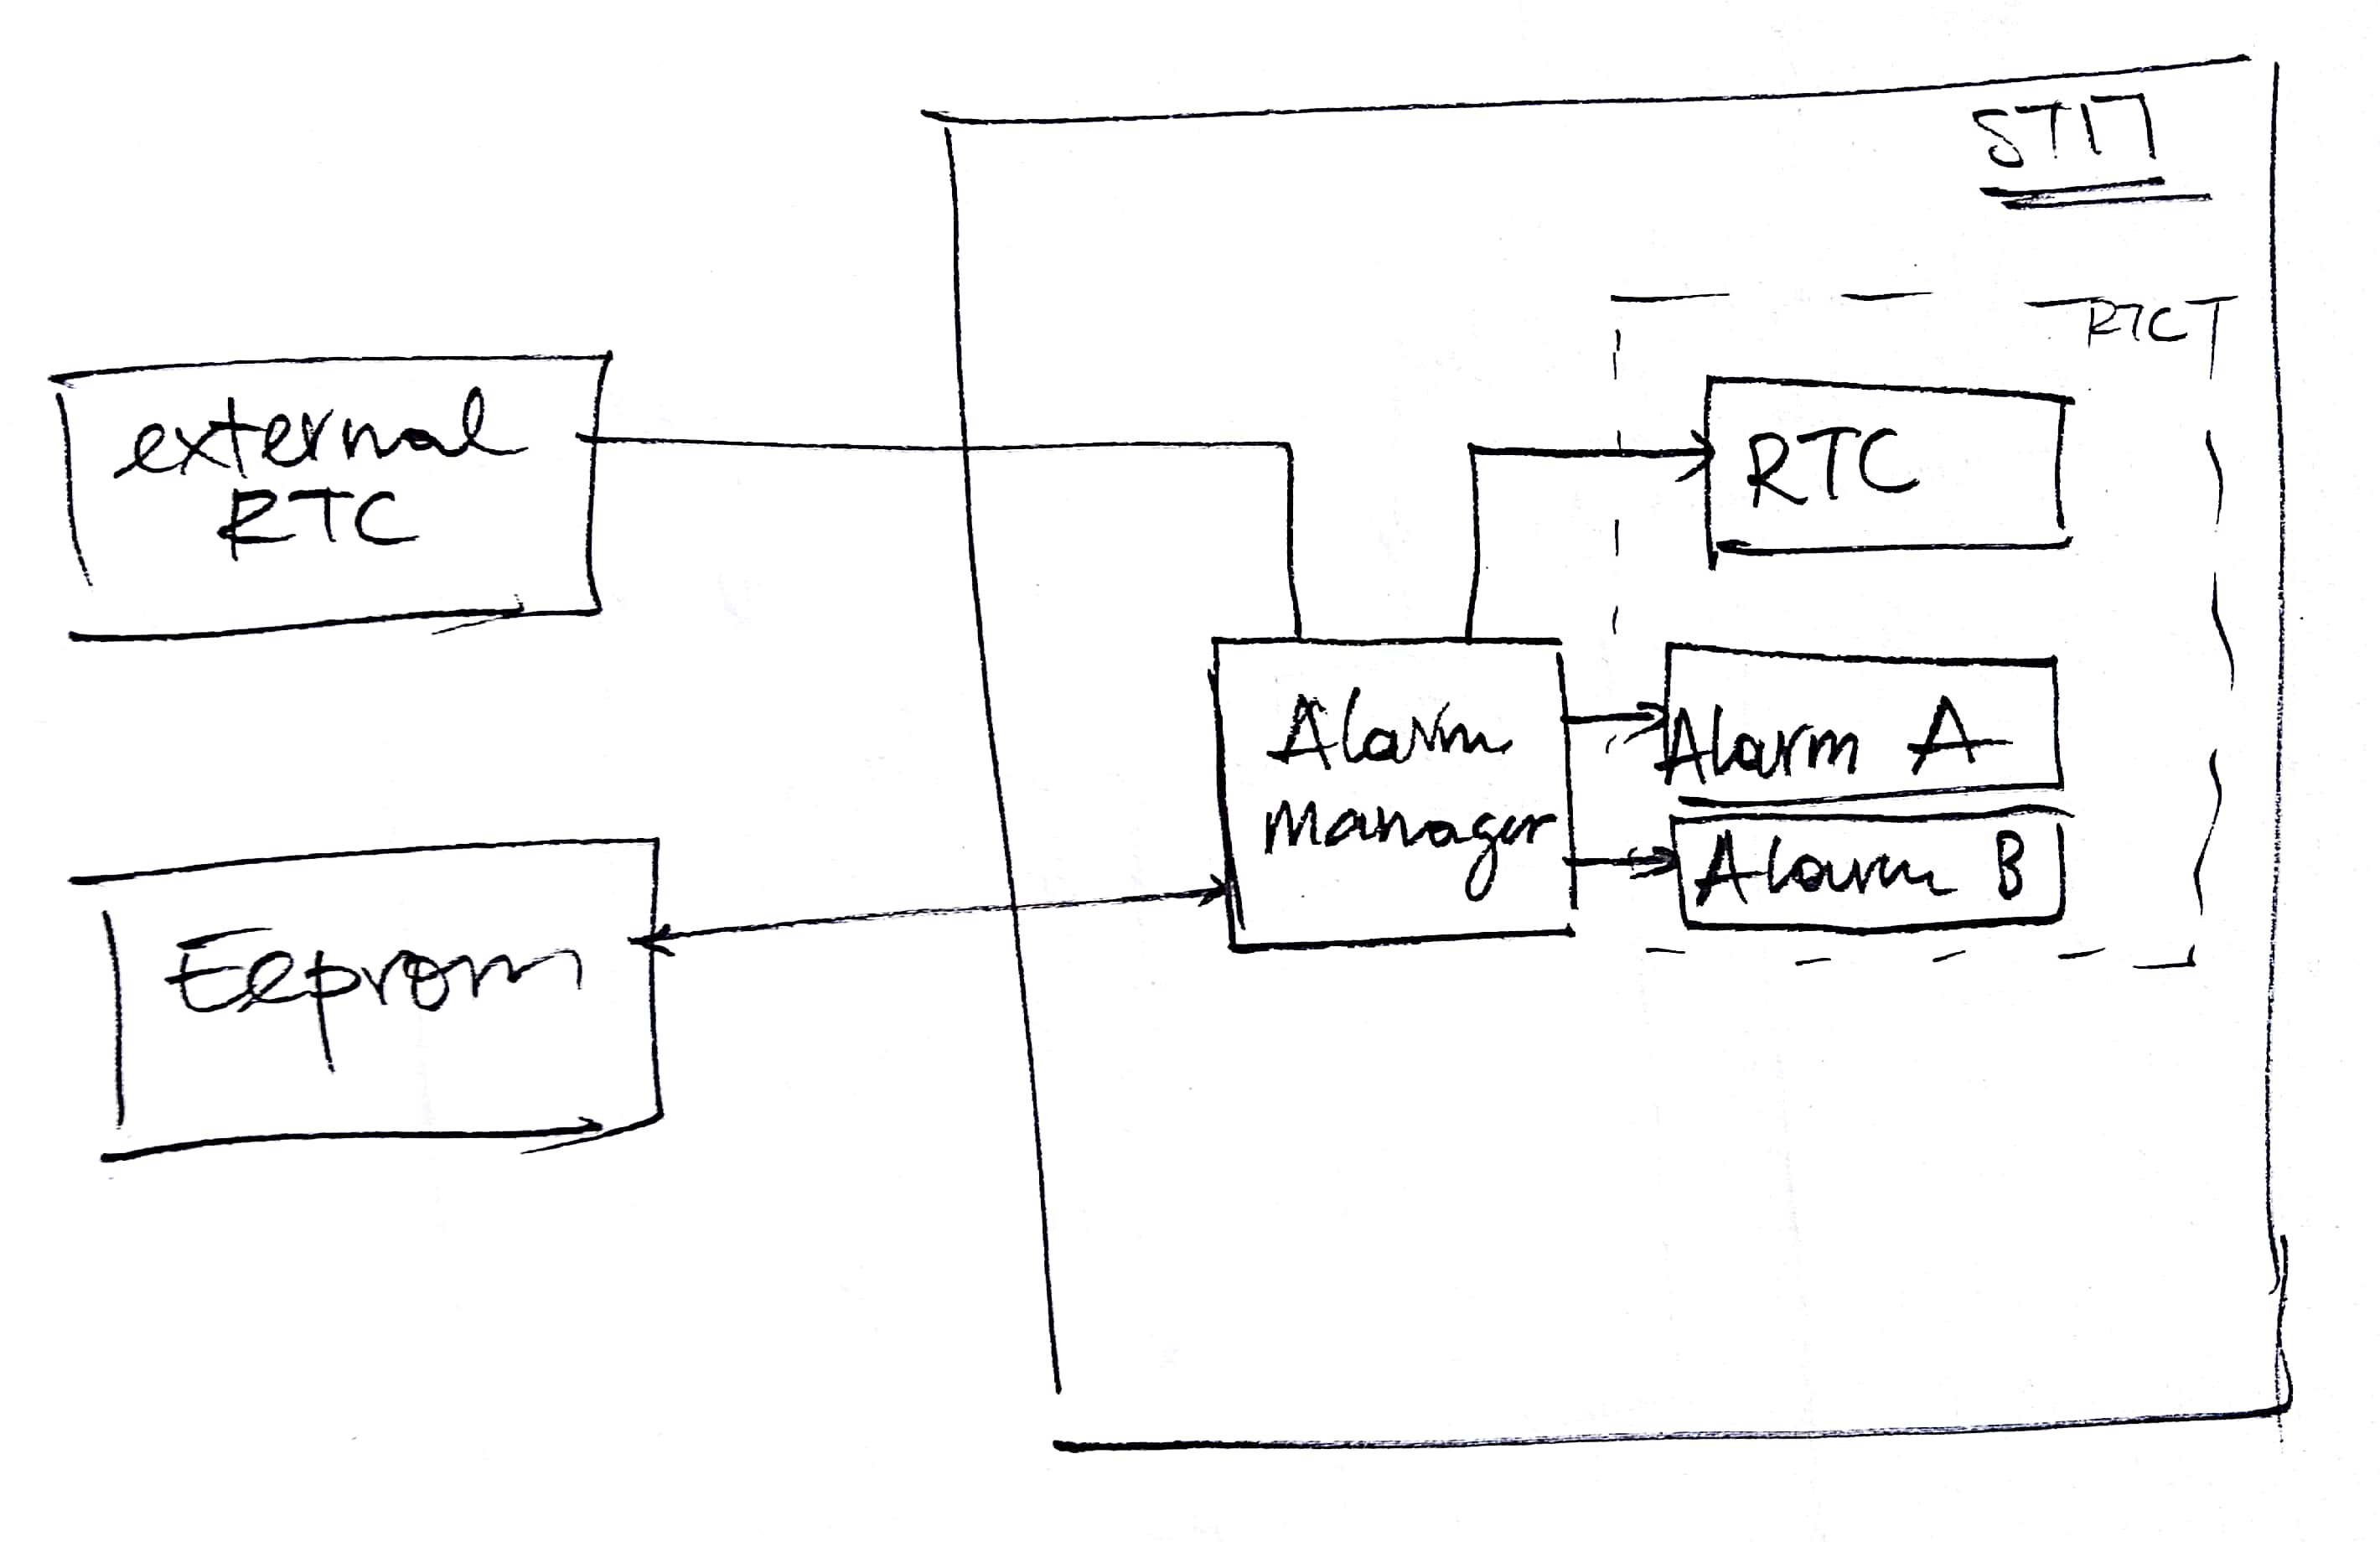
\includegraphics[scale=0.11]{alarm_clock.jpg}
\caption{}
\label{fig:alarm_clock}
\end{figure}
Alarm A and B are triggered based on the comparison of their time with the internal RTC of the STM. As for the internal (built-in) RTC, it relies on the crystal oscillator of the STM to update its time. This RTC is power dependent and loses its time when the STM is powered off. To prevent manual update of the time everytime the STM is powered on, an external clock module must be used. For this prototype, the DS1307 RTC is used as the external clock module. This RTC is not very accurate, in many applications, it has lost few minutes of accuracy every day. This prototype is a proof of concept and is focused on the light requirements and not the accuracy of the clock, therefore, the DS1307 will be used. Later versions of the NPSC could use more accuracy clock module such as a GPS or more accurate RTC.  \\
On power on, the Alarm manager synchronises the internal clock with the external clock by loading the external RTC's time and date to the internal RTC. It then loads two alarms from the EEPROM which are supposed to be triggered before the others and set these alarms to alarm A and alarm B from the internal RTC. The Alarm manager is also responsible for storing the alarms to the EEPROM and updating then when an alarm goes off. 

\subsection{Visual outputs}
The visual outputs are all modules related to the control and emission of light in the system. \Cref{fig:visual_outputs} illustrates the interaction between these modules and the STM. 
\begin{figure}[ht]
\centering
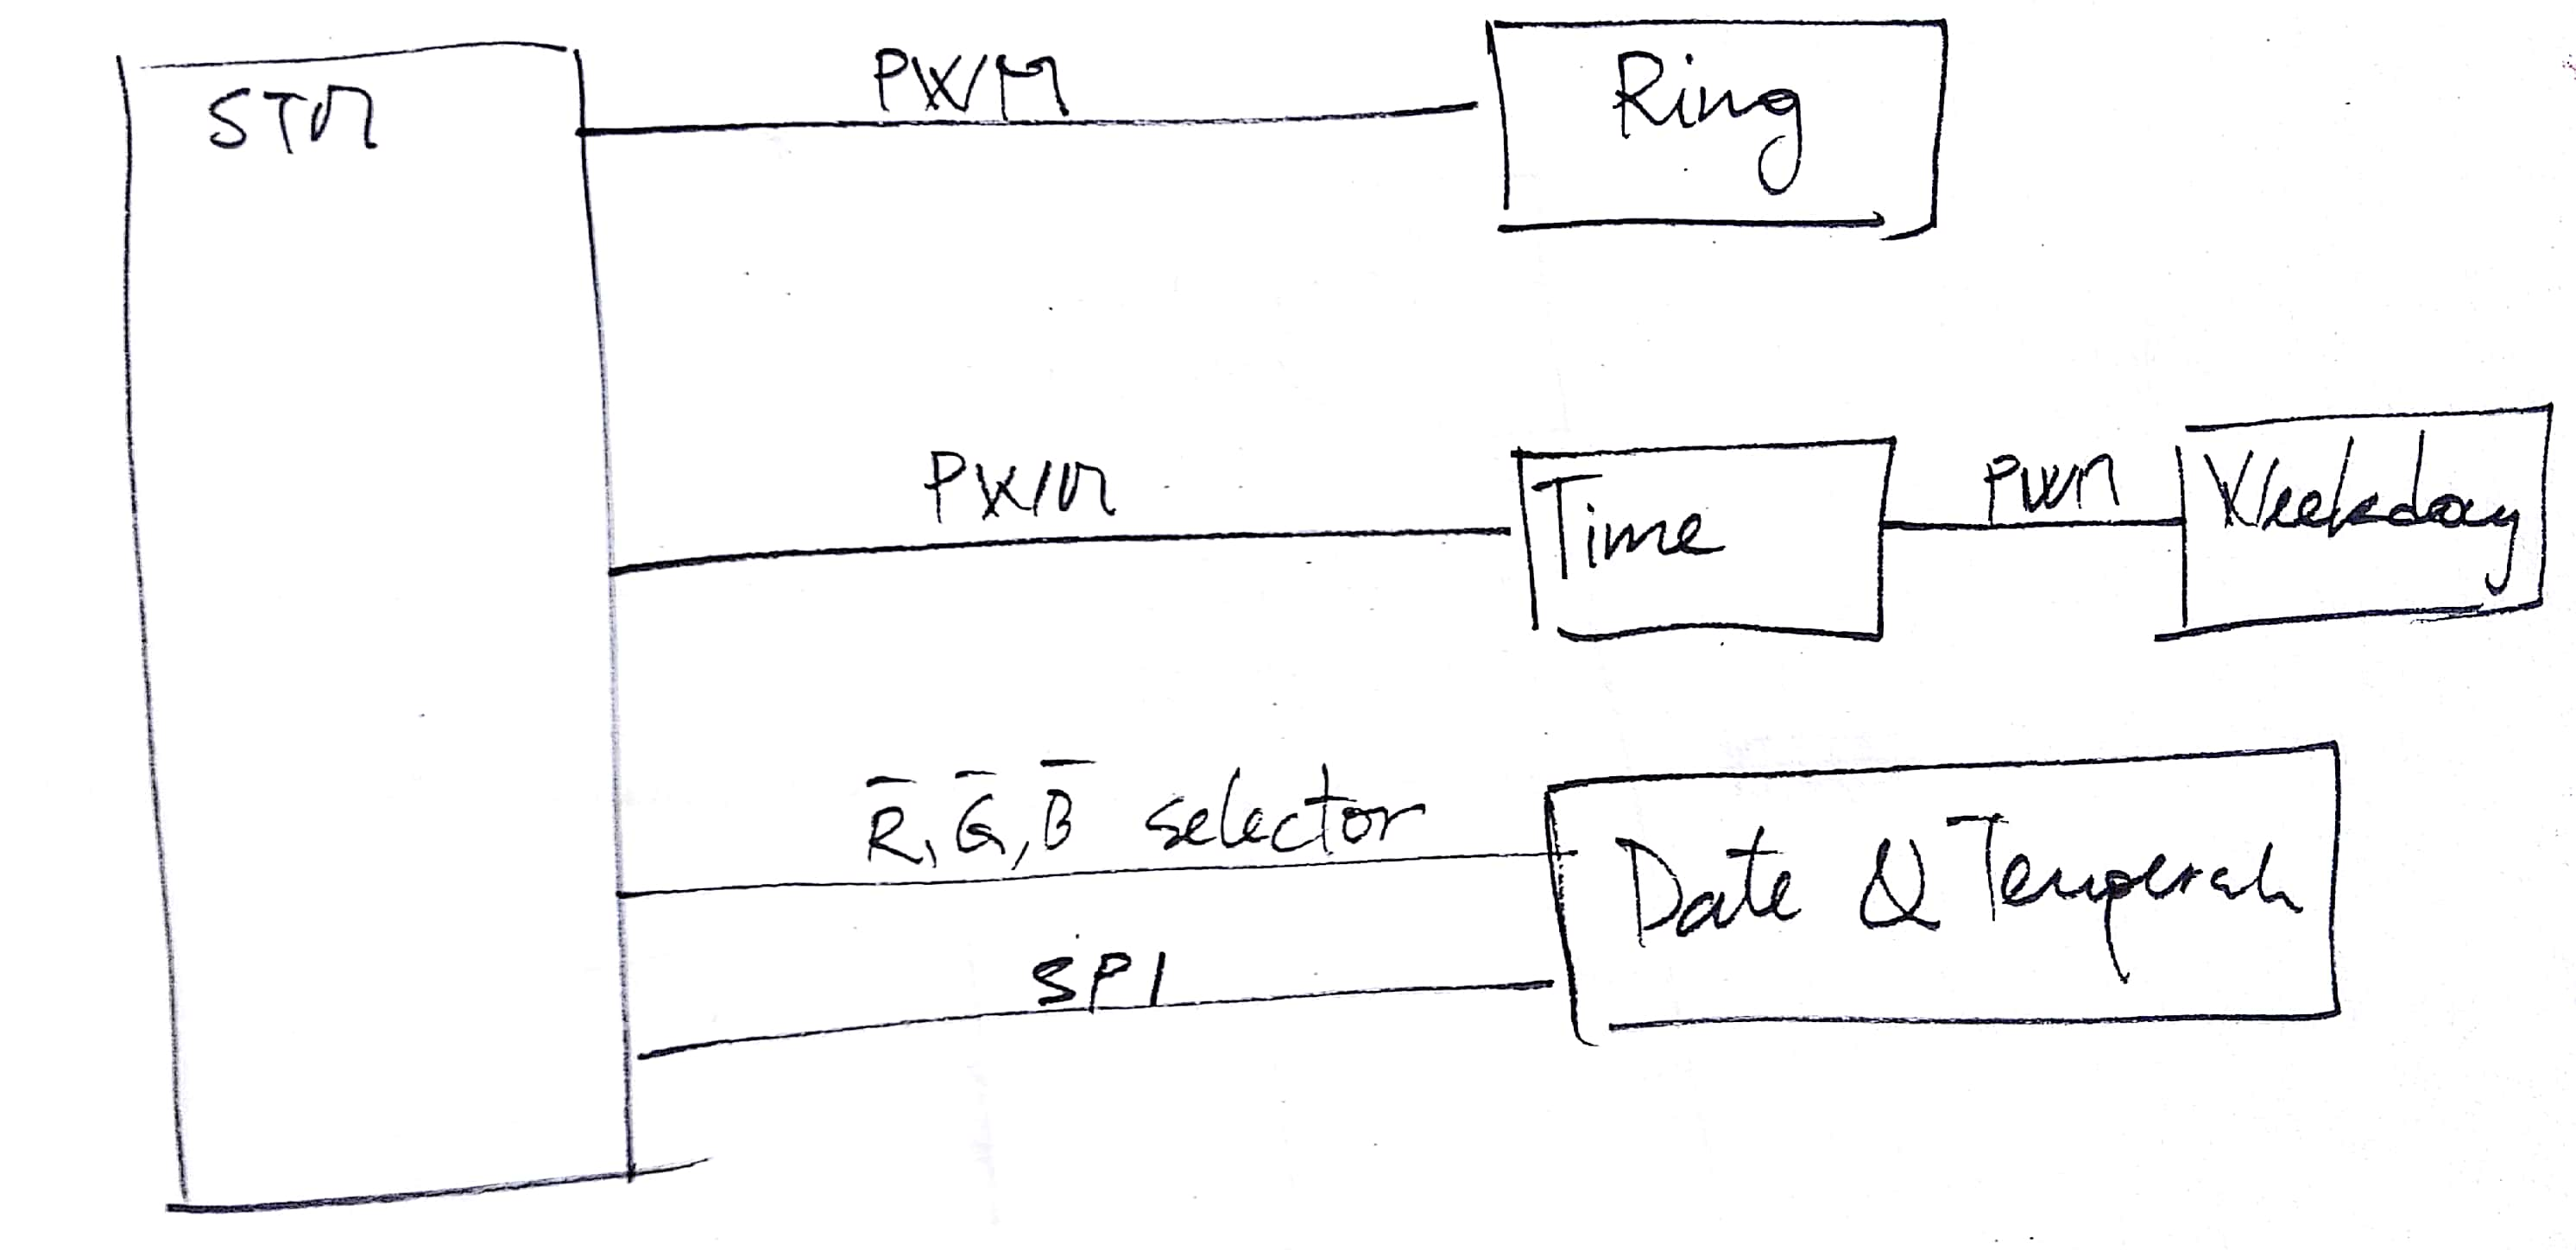
\includegraphics[scale=0.12]{visual_outputs.jpg}
\caption{}
\label{fig:visual_outputs}
\end{figure}
There are two types of hardware modules, the first type (type 1) of modules is a series of neopixels connected in cascade controlled by Pulse Width Modulation (PWM), the second type (type 2) of modules are controlled using a Serial Peripheral Interface (SPI) bus. All type 1 modules inherit the ability to be connected in cascade from the neopixels; however, the ring is the only light source used to affect the human sleep-wake cycle, it is essential that its control is separated from another type 1 module. The two other type 1 is designed to display time and date information, therefore, they can be combined as one module. The only type 2 module in the visual outputs is the Date PCB, this PCB is designed to display the date, the month and the room temperature.\\
For consistency in the visual, RGB 7 segments displays are used for the Date PCB. Moreover, the Time PCB uses neopixels as no RGB 7 segments displays bigger than the ones used for the Date PCB could be found.\\
The visual outputs are controlled by the Visual manager from the visual application. The Visual manager's role is to update the neopixel buffer for each type 1 module according to the visual parameters set by the user. These parameters consist of RGB colours, the brightness, the location of the pixel \footnote{The location is the number of the neopixel of interest in the series of neopixel on a specific module. On the Ring PCB, location 61 is the first neopixel on the second ring.}. At a higher level of control, these parameters also include module's pattern, mode and duration. The Visual manager is also responsible for updating information on the Date PCB.   

\subsection{Sensors}
There are two sensors on the NPSC, a temperature sensor and a photoresistor. The role of the temperature sensor is to get the room temperature. The photoresistor has a more interesting purpose; it is used to obtain the light intensity outside the NPSC in order to allow the system to adjust the neopixel brightness such that the required illuminance does not vary by a significant margin at the user's location.



%%%%%%%%%%%%%%%%%%%%%%%%%%%%%%%%%%%%%%%%%%%%%%%%%%%%%%%%%%%%%%%%%%%%%%%%%%%%%%%%%%%%
% SECTION: Detailed design
%%%%%%%%%%%%%%%%%%%%%%%%%%%%%%%%%%%%%%%%%%%%%%%%%%%%%%%%%%%%%%%%%%%%%%%%%%%%%%%%%%%%
\section{Details hardware design} \label{design}
This section provides detailed information on the design of the hardware modules. Off the shelves, hardware modules are not detailed in this sections as these modules already have the necessary information on their datasheets. All datasheets are in \ref{datasheets} and in the repository on GitHub. 

\subsection{Neopixels boards}
The type 1 modules are made up of series neopixels connected in a daisy chain fashion. Each neopixel has two power pins and two data pins as illustrated by \cref{fig:neopixel_sch}. The stream of bytes is received by the neopixel at its DIN pin, after extracting the first 24 bytes, the neopixel transmit the truncated stream to the DOUT pin. By connecting the DOUT pin of one neopixel to the DIN pin of the next neopixel, a single stream of bytes can be used to program all neopixels in the series. 
\begin{figure}[ht]
\centering
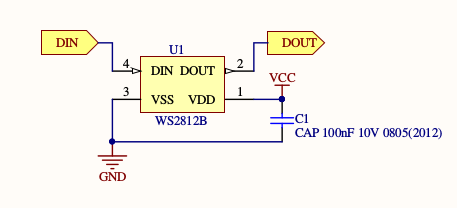
\includegraphics[scale=0.5]{neopixel_sch.png}
\caption{}
\label{fig:neopixel_sch}
\end{figure}
Although all type 1 module uses the sample principle, each module has more specific features in its design.
\subsubsection{Ring PCB}
This module has 180 neopixels physical positioned such that they form three rings of 60 neopixels each. Unlike the neopixel in \cref{fig:neopixel_sch}, there is one capacitor per five neopixels. The daisy chain is broken at every $15^{th}$ neopixels for debugging the data stream. \\
As mentioned in \cref{table:neopixel_specs}, each neopixel requires $20mA$ per colour. The ring uses 180 neopixels thus a current of $20*3*180 = 10800 mA$ is expected to be drawn by the Ring. Following the IPC2221 standard, the board width was calculated with a current of $12A$ (worst case scenario), a board thickness of $1oz/ft^2$ and a temperature rise of $15^oC$; the required trace width of the external layers must be at least\textbf{9.84mm}. This is a stringent requirement on the NPSC as the ring must be contained in a $25*25*10cm^3$ case. With an expected an inner radius of $6.5cm$ and an outer radius of $10.5cm$, the Ring has approximately a surface area of $ \pi*(10.5^2-6.5^2) = 213.63 cm^2$ on each side for dissipating its heat. Furthermore, the neopixel pins have a pad on $0.6*1.5 mm^2$ while the width of the power line must be at least $9.84mm$. Each ring has 60 neopixels thus $60*9.84=$ \textbf{590.4mm} is required as the width of the power line per ring. However, the minimum circumference of the ring is $65*2*\pi$ = \textbf{408.41mm} which is less than what is required. With this conditions, the board is expected to have a higher temperature rise.\\
The schematic and PCB of this board are shown in \cref{fig:ring_sch_pcb}.

\subsubsection{Time}
This board has its series of neopixels physically placed on the board such that they simulate four RGB seven segment display. The board is made generic so that each display can be controlled by its own data pin. The board also has the ability to be controlled all display using the first display controller pin, this is done by connecting the DOUT of the last neopixel of a display to the DIN of the first neopixel in the next display.
The schematic and PCB of this board are shown in \cref{fig:time_sch_pcb}.

\subsubsection{Weekday}
This board has only seven neopixels in its series, one for each day in the week. It gets its input (DIN) from the output (DOUT) of the Time PCB.
The schematic and PCB of this board are shown in \cref{fig:weekday_sch_pcb}.

\subsection{Date and Temperature PCB}
This PCB uses six seven segments display to display the date, the month and the room temperature. \Cref{fig:date} shows the simplified schematic of this module. The seven segment used is the ACD8143 which contain a pair of RGB seven segments display. In order to reduce the number of pins used to control these displays, the serial interfaced 8-digits LED driver display (MAX7219) was used. It uses SPI to control the segments of all the displays. It controls the displays by continuously selecting each display in a loop and setting the segments to the desired voltage. The MAX7219 is not designed for RGB seven segments displays, therefore, additional circuits composed of R, G, B signals and NOT gates were used such that on display selection, the display has the colour set by the R, G, B selectors.   
\begin{figure}[ht]
\centering
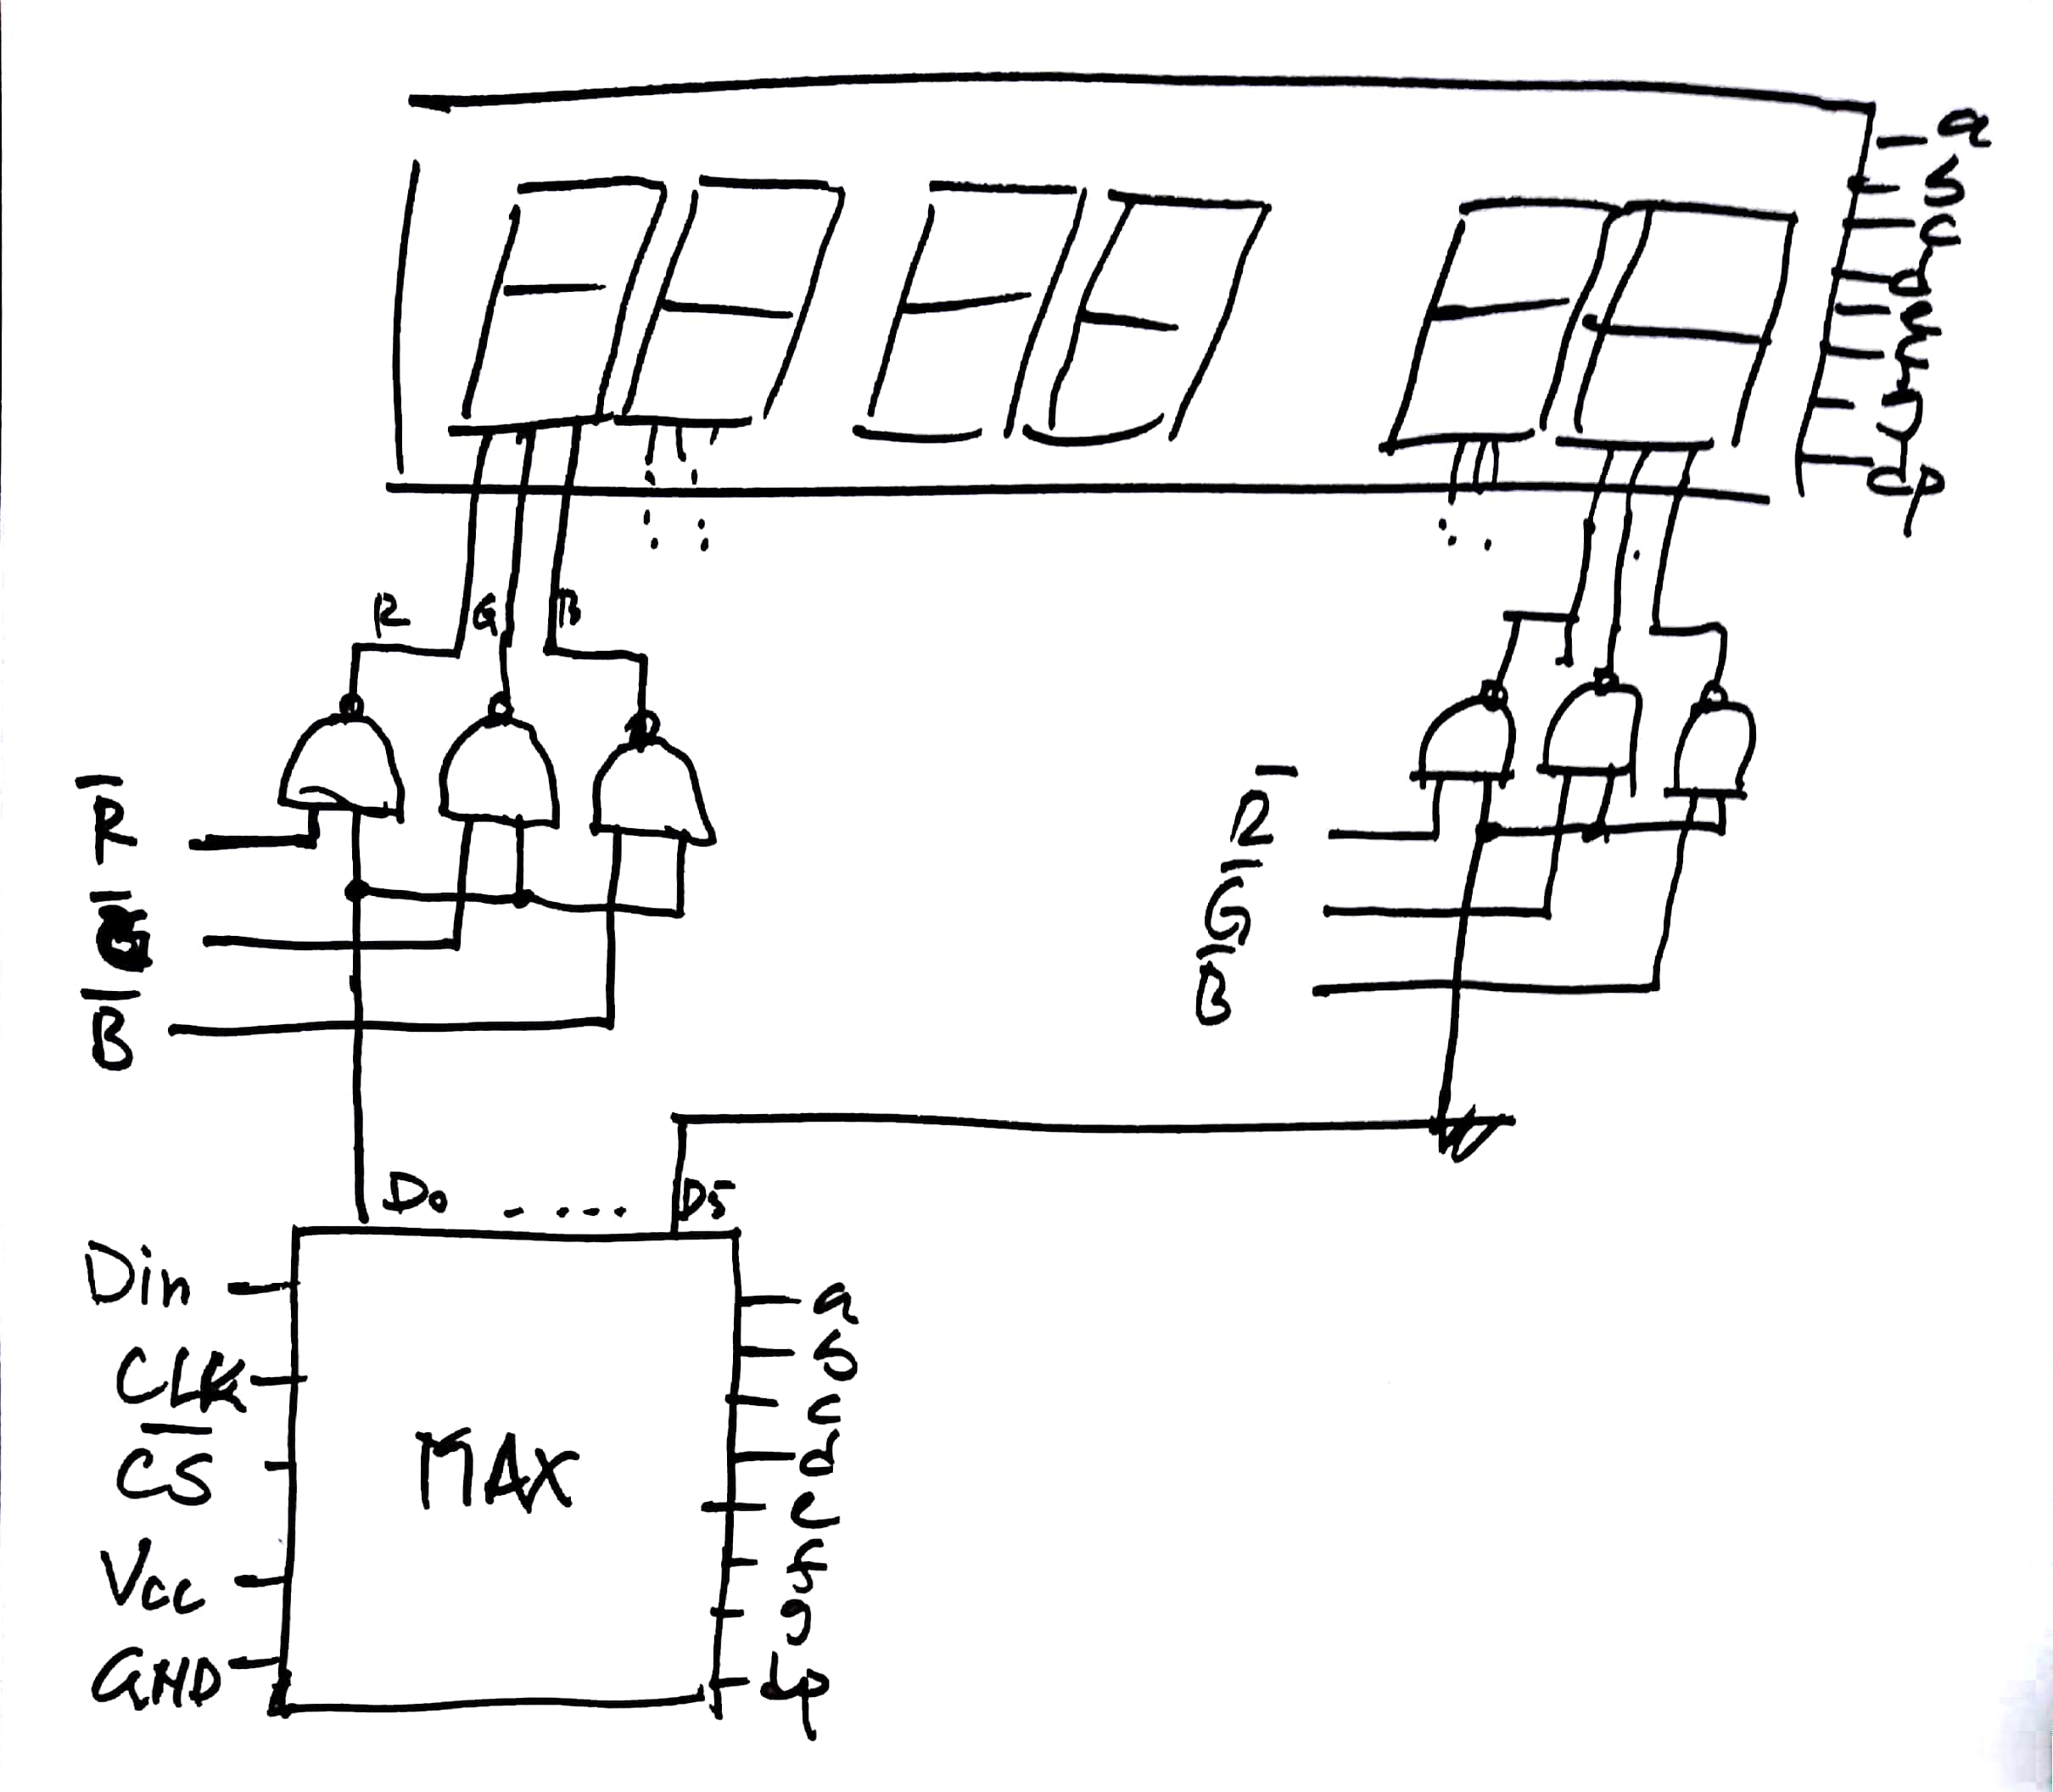
\includegraphics[scale=0.1]{date.jpg}
\caption{}
\label{fig:date}
\end{figure}